\section{Motivation}
The ability to measure changes in the hemoglobin concentration in skin will enable more personalized patient care which, in turn, will lead to an increase in treatment success rates and a decrease in per-patient costs.

For example, in radiation therapy, a common side effect is a skin-reddening reaction known as erythema, or radiation dermatitis.CITATION Erythema is caused by/the result of . . . Depending on the severity of the reaction, erythema can be quite painful and may even prevent the completion of the radiation treatment schedule, thereby reducing the overall treatment efficacy. Unfortunately, since it is a deterministic effect,{citation: Radiation Bio text} with a varying threshold dose and a spectrum of reactions, erythema is impossible to reliably predict in advance. Instead, patients’ responses are monitored by the therapy team over the course of treatment. The current method for monitoring erythema is by visual assessment (VA). VA uses a pre-determined scale to classify the current condition of the skin. If there are too few divisions on the scale (four or less), there is not a sufficient amount of information regarding the patient’s progress from the erythema stage to the next stage of moist desquamation. If there are more than four divisions on the scale, it is difficult to eliminate, or even minimize, the inter- and intra-observer variation, making the results unreliable at best, and preventing any comparison between patients. The implementation of an objective method for measuring skin redness would allow for the treatment team to better manage the reaction, thus improving the treatment’s success rate and the patient’s quality of life.

Other examples where knowledge of the blood concentration of skin would prove beneficial include plastic surgery and burn victims…

\section{Light-tissue interactions}
Jacques \& Patterson, Chapter D.3.1 – Light-tissue interactions
Welch \& Van Gemert, Chapter 2 – Definitions and overviews of tissue optics

\subsection{Reflection}
Specular and diffuse

\subsection{Absorption}
Text

\subsection{Scattering}
Text

\subsection{Other important quantities}
Text

\section{Modeling of light transport in turbid material}
\subsection{Radiation transport equation and diffusion theory}
The radiation transport equation (RTE), also known as the Boltzmann equation, describes the transfer of neutron particles (in this case, energy in the form of photons) within an infinitesimal volume as a function of time.\cite{Duderstadt1976} It is often expressed as a change in the time- and space-resolved energy radiance, $L(\mathbf{r},\mathbf{\Omega},t)$ with respect to time. This quantity can be determined by investigating the mechanism by which the energy radiance can be gained and lost from the volume in question. When considering the steady-state condition, there is no net change in the energy radiance and the gain terms equal the loss terms.

The gain mechanisms are:
\begin{enumerate}
	\item Any photon sources within the volume, $ S(\mathbf{r},\mathbf{\Omega}) $
	\item Photons already within the volume that scatter into the direction of interest,  $\int_{4\pi} L(\mathbf{r},\mathbf{\Omega}) \mu_s(\mathbf{r},\mathbf{\Omega}' \rightarrow \mathbf{\Omega}) d \mathbf{\Omega'} $
	\item Photons that enter into the volume along the direction of interest
\end{enumerate}

Loss mechanisms include:
\begin{enumerate}
	\item Photons that are absorbed within the volume, $ \mu_a L(\mathbf{r},\mathbf{\Omega}) $
	\item Photons that scatter out of the volume, $ \mu_s L(\mathbf{r},\mathbf{\Omega}) $
	\item Photons that exit the volume
\end{enumerate}

A single convection term can be used to account for the photons entering and exiting the volume, $-\mathbf{\Omega}\cdot\nabla L(\mathbf{r},\mathbf{\Omega})$. The combination of all of the terms results in the following equation for the steady-state RTE,\cite{Farrell2003}

\begin{equation}
\label{eq:rte}
\mathbf{\Omega}\cdot\nabla L(\mathbf{r},\mathbf{\Omega}) + (\mu_a + \mu_s) L(\mathbf{r},\mathbf{\Omega}) - \int_{4\pi} L(\mathbf{r},\mathbf{\Omega}) \mu_s(\mathbf{r},\mathbf{\Omega}' \rightarrow \mathbf{\Omega}) d \mathbf{\Omega'} - S(\mathbf{r},\mathbf{\Omega}) = 0
\end{equation}

Solutions to the above equation may be found via intense numerical methods, but they are extremely computationally expensive. As such, a simpler approach is often employed, in which approximations are made that simplify the RTE into a solution-friendly form. In the case of light transport in tissue, the diffusion approximation simplifies the above equation into a single differential equation.
Diffusion theory requires the radiance to be isotropic. This condition is generally met in a semi-infinite medium at a point greater than 1 mfp away from the source or boundaries\cite{Jacques2004} and when $ \mu_a < 0.1\mu_s'$.\cite{Wilson2008} In other words, when the probability of scattering is much greater than the probability of absorption, the direction of the photons is mostly randomized after only a few scattering events, or 1 mfp. The result of these approximations is the diffusion equation as follows,

\begin{equation}
\label{eq:diffeq}
\nabla^2 \cdot \Phi(\mathbf{r}) - \frac{\mu_a}{D}\Phi(\mathbf{r}) = S(\mathbf{r})
\end{equation}

Where $\Phi(\mathbf{r})$ is the energy fluence rate (the integral of the energy radiance over all angles), $D$ is the diffusion constant, $(3\mu_t')^{-1}$, and $S(\mathbf{r})$ is the source term.

The diffusion equation can be solved analytically by applying a set of boundary conditions. In the case of tissue optics, the most common boundary conditions have been developed to account for the mismatch in the index of refraction between the tissue and the air, and the resulting Fresnel reflections from the interior surface of the tissue.

\subsection{Monte Carlo simulations}
Welch \& Van Gemert, Chapter 4 – Monte Carlo..
When diffusion theory cannot be applied, a slightly less computational expensive method of solving the steady-state RTE is via Monte Carlo (MC) simulation.

Stochastic simulation of 

REWORD Mono (or “white”) MC is where there is no absorption (mua=0) during the simulation, only scattering. As a consequence, albedo=0 which means there is no survival weighting. Photon weighting is only modified through interaction with the sphere wall. Photons are only killed when weight is reduced below set level or scatters in tissue many times (via Russian roulette). The total pathlength (s) travelled in tissue of each photon is tracked. When photons are finally scored, the final weight is added to a bin corresponding to the total pathlength. The effect of absorption is introduced by multiplying each bin by EXP(-mua*s) and then summing over all the bins.

Parallelization

\section{1.4	\emph{In vivo} measurements of tissue optical properties with diffuse reflectance}
For the purposes of monitoring patient response, \emph{ex vivo} methods for determining tissue optical properties are obviously not appropriate. Therefore, this section will focus solely on a specific subset of available \emph{in vivo} methods – those that require steady-state conditions, as opposed to time resolved systems.

\subsection{Total diffuse reflectance}
The total diffuse reflectance represents the fraction of the incident light fluence remitted from the tissue across the entire surface (i.e. it is spatially integrated) at a single wavelength. It can be modelled with the diffusion approximation and is dependent only on the reduced albedo and the relative index of refraction.\cite{Kim2011} The index of refraction for skin has been accurately measured, and a value of 1.4 is typically used for incident light within the visible spectrum.\cite{Kienle1996a} With this information, the albedo of the tissue can be determined from the measured total diffuse reflectance. For a single total diffuse reflectance measurement, there is no way of determining the individual contributions from scattering and absorption. However, if the scattering and mean pathlength are assumed constant, a second measurement, where the absorption coefficient is known or can be approximated, will allow for the determination of the other absorption coefficient. This technique relies on the relationship between the total diffuse reflectance and the exponential of the absorption coefficient and the pathlength. The total diffuse reflectance is generally measured either with an integrating sphere (see Section~\ref{sec:is_theory}) or with an optical system, off-set from the normal to avoid collecting any specular reflection.

\subsection{Spatially-resolved diffuse reflectance}
The spatially-resolved diffuse reflectance is the fraction of the incident light remitted at a specific radial distance from the incident light source. It is collected by detection fibers positioned at many (at least two) distances from the source fiber.\cite{Kim2011} To maintain accurate positioning, the source and detection fibers are usually bundled together in a single probe. To improve the signal-to-noise ratio, several probes are used at greater distances (see Figure~\ref{fig:intro-srdr}).

\begin{figure}
	\centering 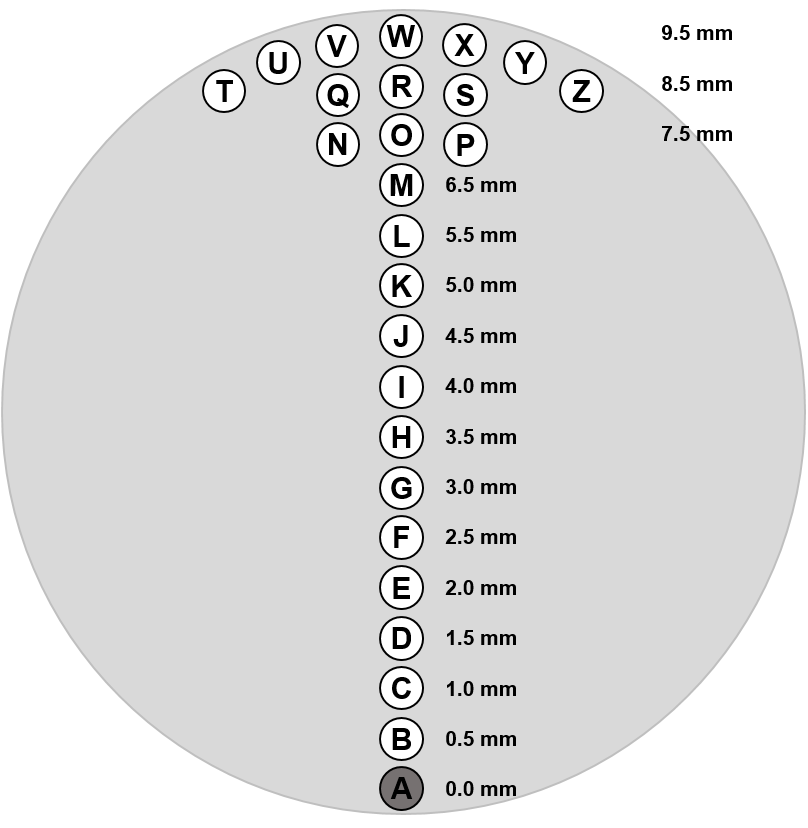
\includegraphics[width=0.5\textwidth]{figures/intro-srdr.png}
	\caption[Probe for spatially-resolved diffuse reflectance]{\label{fig:intro-srdr}A diagram representing the configuration of the optical fibers in the probe. Light enters through fibre “A” (dark grey) and is detected by additional fibers that are placed set distances away (white).}
\end{figure}

Both the absorption and reduced scattering coefficients can be determined with this method. The first step is to determine the effective attenuation coefficient, which is approximated by the terminal slope of the curve of $\ln[r^m R_d(r)] $ as a function of the radial distance. Next, the measurements from all of the detector probes can be collected to produce the total diffuse reflectance which can yield the albedo. Together, these two quantities (the effective attenuation coefficient and the albedo) can then be combined to obtain the absorption and reduced scattering coefficient.

\subsection{Spectrally-constrained diffuse reflectance}
A recently popular method is to use a single source-detector pair instead of a spatially-resolved array of detector fibers. This approach employs a broad beam light source instead of a single wavelength light source, and resolves the collected signal into a reflectance measurement at each wavelength. However, this reflectance spectrum is not sufficient and additional information is required to determine the tissue optical properties. A spectrally-constrained solution requires assumptions about the shapes of the absorption and reduced scattering coefficient spectra.

\section{Integrating sphere theory}
\label{sec:is_theory}
Text

\section{Human skin}
Human skin consists of two layers: the epidermis and the dermis.CITATION The epidermis is the top-most layer of skin. As shown in Figure~\ref{fig:intro-skin_layers}, Keratinocytes (skin cells) are produced at the deepest section of the epidermis in the stratum basale and migrate toward the surface, through the statum spinosum and the stratum granulosum to the stratum corneum, losing their internal structures and organelles during the process. The stratum corneum (the skin surface) consists of dead, mature keratinocytes which are easily shed. Also found in the epidermis are melanocytes, the melanin-producing cells which are majorly responsible for skin color. The average epidermal thickness is less than 1 mm.\cite{Huclova2012}

\begin{figure}
	\centering 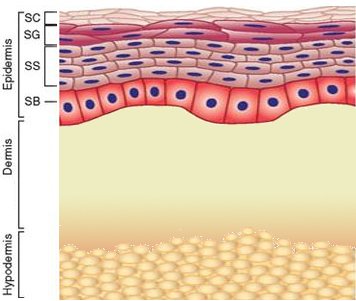
\includegraphics[width=0.5\textwidth]{figures/intro-skin_layers.jpg}
	\caption[Hover text]{\label{fig:intro-skin_layers}Actual caption text goes here.}
\end{figure}

The second layer of skin is the dermis. It contains mostly collagen and elastic fibers but is also the location of capillaries and some nerves. The average dermal thickness is approximately 1.5 mm but can vary widely depending on the site.

Below the skin is the subcutaneous layer, also known as the hypodermis or subcutis. The thickness of this layer varies greatly because this is the layer that contains subcutaneous fat. This is also the location of the majority of superficial veins which can occasionally be visible at the surface. A representative thickness for this layer is 5 mm.

Chromophores

Discuss how deep visible light may penetrate?

Anatomy, constituent chromophores, physiology (blanching, reddening)

Tissue perfusion, vasoconstriction, vasodilation

Tissue oxygen saturation (StO2) is related to blood flow (citation: McNaulty, 2011)

\section{Thesis proposal}